% Options for packages loaded elsewhere
\PassOptionsToPackage{unicode}{hyperref}
\PassOptionsToPackage{hyphens}{url}
%
\documentclass[
]{article}
\usepackage{amsmath,amssymb}
\usepackage{lmodern}
\usepackage{iftex}
\ifPDFTeX
  \usepackage[T1]{fontenc}
  \usepackage[utf8]{inputenc}
  \usepackage{textcomp} % provide euro and other symbols
\else % if luatex or xetex
  \usepackage{unicode-math}
  \defaultfontfeatures{Scale=MatchLowercase}
  \defaultfontfeatures[\rmfamily]{Ligatures=TeX,Scale=1}
\fi
% Use upquote if available, for straight quotes in verbatim environments
\IfFileExists{upquote.sty}{\usepackage{upquote}}{}
\IfFileExists{microtype.sty}{% use microtype if available
  \usepackage[]{microtype}
  \UseMicrotypeSet[protrusion]{basicmath} % disable protrusion for tt fonts
}{}
\makeatletter
\@ifundefined{KOMAClassName}{% if non-KOMA class
  \IfFileExists{parskip.sty}{%
    \usepackage{parskip}
  }{% else
    \setlength{\parindent}{0pt}
    \setlength{\parskip}{6pt plus 2pt minus 1pt}}
}{% if KOMA class
  \KOMAoptions{parskip=half}}
\makeatother
\usepackage{xcolor}
\IfFileExists{xurl.sty}{\usepackage{xurl}}{} % add URL line breaks if available
\IfFileExists{bookmark.sty}{\usepackage{bookmark}}{\usepackage{hyperref}}
\hypersetup{
  pdftitle={Replication Code for Figures in A Practical Guide to Dealing with Attrition in Political Science Experiments},
  hidelinks,
  pdfcreator={LaTeX via pandoc}}
\urlstyle{same} % disable monospaced font for URLs
\usepackage[margin=1in]{geometry}
\usepackage{color}
\usepackage{fancyvrb}
\newcommand{\VerbBar}{|}
\newcommand{\VERB}{\Verb[commandchars=\\\{\}]}
\DefineVerbatimEnvironment{Highlighting}{Verbatim}{commandchars=\\\{\}}
% Add ',fontsize=\small' for more characters per line
\usepackage{framed}
\definecolor{shadecolor}{RGB}{248,248,248}
\newenvironment{Shaded}{\begin{snugshade}}{\end{snugshade}}
\newcommand{\AlertTok}[1]{\textcolor[rgb]{0.94,0.16,0.16}{#1}}
\newcommand{\AnnotationTok}[1]{\textcolor[rgb]{0.56,0.35,0.01}{\textbf{\textit{#1}}}}
\newcommand{\AttributeTok}[1]{\textcolor[rgb]{0.77,0.63,0.00}{#1}}
\newcommand{\BaseNTok}[1]{\textcolor[rgb]{0.00,0.00,0.81}{#1}}
\newcommand{\BuiltInTok}[1]{#1}
\newcommand{\CharTok}[1]{\textcolor[rgb]{0.31,0.60,0.02}{#1}}
\newcommand{\CommentTok}[1]{\textcolor[rgb]{0.56,0.35,0.01}{\textit{#1}}}
\newcommand{\CommentVarTok}[1]{\textcolor[rgb]{0.56,0.35,0.01}{\textbf{\textit{#1}}}}
\newcommand{\ConstantTok}[1]{\textcolor[rgb]{0.00,0.00,0.00}{#1}}
\newcommand{\ControlFlowTok}[1]{\textcolor[rgb]{0.13,0.29,0.53}{\textbf{#1}}}
\newcommand{\DataTypeTok}[1]{\textcolor[rgb]{0.13,0.29,0.53}{#1}}
\newcommand{\DecValTok}[1]{\textcolor[rgb]{0.00,0.00,0.81}{#1}}
\newcommand{\DocumentationTok}[1]{\textcolor[rgb]{0.56,0.35,0.01}{\textbf{\textit{#1}}}}
\newcommand{\ErrorTok}[1]{\textcolor[rgb]{0.64,0.00,0.00}{\textbf{#1}}}
\newcommand{\ExtensionTok}[1]{#1}
\newcommand{\FloatTok}[1]{\textcolor[rgb]{0.00,0.00,0.81}{#1}}
\newcommand{\FunctionTok}[1]{\textcolor[rgb]{0.00,0.00,0.00}{#1}}
\newcommand{\ImportTok}[1]{#1}
\newcommand{\InformationTok}[1]{\textcolor[rgb]{0.56,0.35,0.01}{\textbf{\textit{#1}}}}
\newcommand{\KeywordTok}[1]{\textcolor[rgb]{0.13,0.29,0.53}{\textbf{#1}}}
\newcommand{\NormalTok}[1]{#1}
\newcommand{\OperatorTok}[1]{\textcolor[rgb]{0.81,0.36,0.00}{\textbf{#1}}}
\newcommand{\OtherTok}[1]{\textcolor[rgb]{0.56,0.35,0.01}{#1}}
\newcommand{\PreprocessorTok}[1]{\textcolor[rgb]{0.56,0.35,0.01}{\textit{#1}}}
\newcommand{\RegionMarkerTok}[1]{#1}
\newcommand{\SpecialCharTok}[1]{\textcolor[rgb]{0.00,0.00,0.00}{#1}}
\newcommand{\SpecialStringTok}[1]{\textcolor[rgb]{0.31,0.60,0.02}{#1}}
\newcommand{\StringTok}[1]{\textcolor[rgb]{0.31,0.60,0.02}{#1}}
\newcommand{\VariableTok}[1]{\textcolor[rgb]{0.00,0.00,0.00}{#1}}
\newcommand{\VerbatimStringTok}[1]{\textcolor[rgb]{0.31,0.60,0.02}{#1}}
\newcommand{\WarningTok}[1]{\textcolor[rgb]{0.56,0.35,0.01}{\textbf{\textit{#1}}}}
\usepackage{graphicx}
\makeatletter
\def\maxwidth{\ifdim\Gin@nat@width>\linewidth\linewidth\else\Gin@nat@width\fi}
\def\maxheight{\ifdim\Gin@nat@height>\textheight\textheight\else\Gin@nat@height\fi}
\makeatother
% Scale images if necessary, so that they will not overflow the page
% margins by default, and it is still possible to overwrite the defaults
% using explicit options in \includegraphics[width, height, ...]{}
\setkeys{Gin}{width=\maxwidth,height=\maxheight,keepaspectratio}
% Set default figure placement to htbp
\makeatletter
\def\fps@figure{htbp}
\makeatother
\setlength{\emergencystretch}{3em} % prevent overfull lines
\providecommand{\tightlist}{%
  \setlength{\itemsep}{0pt}\setlength{\parskip}{0pt}}
\setcounter{secnumdepth}{-\maxdimen} % remove section numbering
\ifLuaTeX
  \usepackage{selnolig}  % disable illegal ligatures
\fi

\title{Replication Code for Figures in
\texttt{A\ Practical\ Guide\ to\ Dealing\ with\ Attrition\ in\ Political\ Science\ Experiments}}
\author{}
\date{\vspace{-2.5em}This version: September 2022}

\begin{document}
\maketitle

Code to replicate figures from the paper A Practical Guide to Dealing
with Attrition in Political Science Experiments by Adeline Lo, Jonathan
Renshon, and Lotem Bassan-Nygate.

\hypertarget{fiure-1-experimental-papers-in-fulljepscorpus-and-their-discussion-of-attrition}{%
\section{Fiure 1: Experimental papers in fullJEPScorpus and their
discussion of
attrition}\label{fiure-1-experimental-papers-in-fulljepscorpus-and-their-discussion-of-attrition}}

\begin{Shaded}
\begin{Highlighting}[]
\CommentTok{\#Reading in CSV Data}
\NormalTok{attrition }\OtherTok{\textless{}{-}} \FunctionTok{read\_csv}\NormalTok{(}\StringTok{"lit\_review.csv"}\NormalTok{)}


\CommentTok{\#Functions to remove "*" and change "Yes" to 1 and "No" to 0}
\NormalTok{remove\_star }\OtherTok{\textless{}{-}} \ControlFlowTok{function}\NormalTok{(x) \{}
  \FunctionTok{return}\NormalTok{(}\FunctionTok{str\_extract}\NormalTok{(x, }\StringTok{"Yes|No"}\NormalTok{))}
\NormalTok{\}}

\NormalTok{yesno\_onezero }\OtherTok{\textless{}{-}} \ControlFlowTok{function}\NormalTok{(x) \{}
  \FunctionTok{return}\NormalTok{(}\FunctionTok{case\_when}\NormalTok{(x }\SpecialCharTok{==} \StringTok{"Yes"} \SpecialCharTok{\textasciitilde{}} \DecValTok{1}\NormalTok{,}
\NormalTok{                   x }\SpecialCharTok{==} \StringTok{"No"} \SpecialCharTok{\textasciitilde{}} \DecValTok{0}\NormalTok{))}
\NormalTok{\}}

\NormalTok{attrition }\OtherTok{\textless{}{-}}\NormalTok{ attrition }\SpecialCharTok{\%\textgreater{}\%} 
  \FunctionTok{mutate\_at}\NormalTok{(}\FunctionTok{c}\NormalTok{(}\DecValTok{7}\SpecialCharTok{:}\DecValTok{14}\NormalTok{), remove\_star) }\SpecialCharTok{\%\textgreater{}\%}
  \FunctionTok{mutate\_at}\NormalTok{(}\FunctionTok{c}\NormalTok{(}\DecValTok{7}\SpecialCharTok{:}\DecValTok{14}\NormalTok{), yesno\_onezero)}


\CommentTok{\#Creating table of proportions}
\NormalTok{prop\_att }\OtherTok{\textless{}{-}} \FunctionTok{mean}\NormalTok{(attrition}\SpecialCharTok{$}\NormalTok{Attrition)}
\NormalTok{prop\_noatt }\OtherTok{\textless{}{-}} \FunctionTok{mean}\NormalTok{(attrition}\SpecialCharTok{$}\StringTok{\textasciigrave{}}\AttributeTok{0 Attrition}\StringTok{\textasciigrave{}}\NormalTok{[attrition}\SpecialCharTok{$}\NormalTok{Attrition }\SpecialCharTok{==} \DecValTok{1}\NormalTok{])}
\NormalTok{prop\_attdv }\OtherTok{\textless{}{-}} \FunctionTok{mean}\NormalTok{(attrition}\SpecialCharTok{$}\StringTok{\textasciigrave{}}\AttributeTok{Response Rate DV}\StringTok{\textasciigrave{}}\NormalTok{[attrition}\SpecialCharTok{$}\NormalTok{Attrition }\SpecialCharTok{==} \DecValTok{1}\NormalTok{])}
\NormalTok{prop\_quan }\OtherTok{\textless{}{-}} \FunctionTok{mean}\NormalTok{(attrition}\SpecialCharTok{$}\StringTok{\textasciigrave{}}\AttributeTok{Quantified Attrition}\StringTok{\textasciigrave{}}\NormalTok{[attrition}\SpecialCharTok{$}\NormalTok{Attrition }\SpecialCharTok{==} \DecValTok{1} \SpecialCharTok{\&}\NormalTok{ attrition}\SpecialCharTok{$}\StringTok{\textasciigrave{}}\AttributeTok{0 Attrition}\StringTok{\textasciigrave{}} \SpecialCharTok{==} \DecValTok{0} \SpecialCharTok{\&}\NormalTok{ attrition}\SpecialCharTok{$}\StringTok{\textasciigrave{}}\AttributeTok{Response Rate DV}\StringTok{\textasciigrave{}} \SpecialCharTok{==} \DecValTok{0}\NormalTok{])}
\NormalTok{prop\_adj }\OtherTok{\textless{}{-}} \FunctionTok{mean}\NormalTok{(attrition}\SpecialCharTok{$}\StringTok{\textasciigrave{}}\AttributeTok{Sample Adjustments}\StringTok{\textasciigrave{}}\NormalTok{[attrition}\SpecialCharTok{$}\NormalTok{Attrition }\SpecialCharTok{==} \DecValTok{1} \SpecialCharTok{\&}\NormalTok{ attrition}\SpecialCharTok{$}\StringTok{\textasciigrave{}}\AttributeTok{0 Attrition}\StringTok{\textasciigrave{}} \SpecialCharTok{==} \DecValTok{0} \SpecialCharTok{\&}\NormalTok{ attrition}\SpecialCharTok{$}\StringTok{\textasciigrave{}}\AttributeTok{Response Rate DV}\StringTok{\textasciigrave{}} \SpecialCharTok{==} \DecValTok{0}\NormalTok{])}

\NormalTok{attrition\_summary }\OtherTok{\textless{}{-}} \FunctionTok{as\_tibble}\NormalTok{(}\FunctionTok{data.frame}\NormalTok{(}
  \FunctionTok{c}\NormalTok{(}\StringTok{"Measurement"}\NormalTok{,}
    \StringTok{"Proportion that mention attrition"}\NormalTok{,}
    \StringTok{"Proportion }\SpecialCharTok{\textbackslash{}"}\StringTok{no attrition}\SpecialCharTok{\textbackslash{}"}\StringTok{"}\NormalTok{,}
    \StringTok{"Proportion DV"}\NormalTok{,}
    \StringTok{"Proportion quantify"}\NormalTok{,}
    \StringTok{"Proportion adjust"}\NormalTok{),}
  \FunctionTok{c}\NormalTok{(}\StringTok{"Value"}\NormalTok{,}
\NormalTok{    prop\_att,}
\NormalTok{    prop\_noatt,}
\NormalTok{    prop\_attdv,}
\NormalTok{    prop\_quan,}
\NormalTok{    prop\_adj)}
\NormalTok{))}


\CommentTok{\#Creating variable for the waffle plot}
\NormalTok{count }\OtherTok{\textless{}{-}}\NormalTok{ attrition }\SpecialCharTok{\%\textgreater{}\%} 
  \FunctionTok{mutate}\NormalTok{(}\AttributeTok{waffle =} \FunctionTok{case\_when}\NormalTok{(}\StringTok{\textasciigrave{}}\AttributeTok{Sample Adjustments}\StringTok{\textasciigrave{}} \SpecialCharTok{==} \DecValTok{1} \SpecialCharTok{\textasciitilde{}} \StringTok{"Attrition mentioned, quantified, analyzed"}\NormalTok{,}
\NormalTok{                            Attrition }\SpecialCharTok{==} \DecValTok{1} \SpecialCharTok{\&} \StringTok{\textasciigrave{}}\AttributeTok{0 Attrition}\StringTok{\textasciigrave{}} \SpecialCharTok{==} \DecValTok{0} \SpecialCharTok{\&} \StringTok{\textasciigrave{}}\AttributeTok{Response Rate DV}\StringTok{\textasciigrave{}} \SpecialCharTok{==} \DecValTok{0} \SpecialCharTok{\&} \StringTok{\textasciigrave{}}\AttributeTok{Sample Adjustments}\StringTok{\textasciigrave{}} \SpecialCharTok{==} \DecValTok{0} \SpecialCharTok{\&} \StringTok{\textasciigrave{}}\AttributeTok{Quantified Attrition}\StringTok{\textasciigrave{}} \SpecialCharTok{==} \DecValTok{1} \SpecialCharTok{\textasciitilde{}} \StringTok{"Attrition mentioned and quantified"}\NormalTok{,}
\NormalTok{                            Attrition }\SpecialCharTok{==} \DecValTok{1} \SpecialCharTok{\&} \StringTok{\textasciigrave{}}\AttributeTok{0 Attrition}\StringTok{\textasciigrave{}} \SpecialCharTok{==} \DecValTok{0} \SpecialCharTok{\&} \StringTok{\textasciigrave{}}\AttributeTok{Response Rate DV}\StringTok{\textasciigrave{}} \SpecialCharTok{==} \DecValTok{0} \SpecialCharTok{\&} \StringTok{\textasciigrave{}}\AttributeTok{Sample Adjustments}\StringTok{\textasciigrave{}} \SpecialCharTok{==} \DecValTok{0} \SpecialCharTok{\&} \StringTok{\textasciigrave{}}\AttributeTok{Quantified Attrition}\StringTok{\textasciigrave{}} \SpecialCharTok{==} \DecValTok{0} \SpecialCharTok{\textasciitilde{}} \StringTok{"Attrition mentioned only"}\NormalTok{,}
                            \StringTok{\textasciigrave{}}\AttributeTok{Response Rate DV}\StringTok{\textasciigrave{}} \SpecialCharTok{==} \DecValTok{1} \SpecialCharTok{\textasciitilde{}} \StringTok{"Attrition is DV"}\NormalTok{,}
                            \StringTok{\textasciigrave{}}\AttributeTok{0 Attrition}\StringTok{\textasciigrave{}} \SpecialCharTok{==} \DecValTok{1} \SpecialCharTok{\textasciitilde{}} \StringTok{"Attrition mentioned {-} none in study"}\NormalTok{,}
\NormalTok{                            Attrition }\SpecialCharTok{==} \DecValTok{0} \SpecialCharTok{\textasciitilde{}} \StringTok{"No mention of attrition"}\NormalTok{)) }\SpecialCharTok{\%\textgreater{}\%} 
  \FunctionTok{group\_by}\NormalTok{(waffle) }\SpecialCharTok{\%\textgreater{}\%}
  \FunctionTok{summarise}\NormalTok{(}\AttributeTok{n =} \FunctionTok{n}\NormalTok{())}

\CommentTok{\#Reordering to make legend easier to read and plot look better}
\NormalTok{count }\OtherTok{\textless{}{-}}\NormalTok{ count[}\FunctionTok{c}\NormalTok{(}\DecValTok{5}\NormalTok{,}\DecValTok{3}\NormalTok{,}\DecValTok{2}\NormalTok{,}\DecValTok{4}\NormalTok{,}\DecValTok{1}\NormalTok{,}\DecValTok{6}\NormalTok{),]}

\CommentTok{\#Creating waffle plot}
\NormalTok{case\_counts }\OtherTok{\textless{}{-}}\NormalTok{ count}\SpecialCharTok{$}\NormalTok{n}
\FunctionTok{names}\NormalTok{(case\_counts) }\OtherTok{\textless{}{-}}\NormalTok{ count}\SpecialCharTok{$}\NormalTok{waffle}

\FunctionTok{waffle}\NormalTok{(case\_counts, }\AttributeTok{colors =} \FunctionTok{c}\NormalTok{(}
  \StringTok{"\#fcba03"}\NormalTok{, }\CommentTok{\#For Attrition mentioned, quantified, analyzed}
  \StringTok{"\#e8803f"}\NormalTok{, }\CommentTok{\#For Attrition mentioned and quantified}
  \StringTok{"\#965ef7"}\NormalTok{, }\CommentTok{\#For Attrition mentioned, none in study}
  \StringTok{"\#595959"}\NormalTok{, }\CommentTok{\#For Attrition mentioned only}
  \StringTok{"\#5eccf7"}\NormalTok{, }\CommentTok{\#For Attrition is DV}
  \StringTok{"\#ff6666"}  \CommentTok{\#For No mention of attrition}
\NormalTok{  )) }\SpecialCharTok{+}
  \FunctionTok{theme}\NormalTok{(}\AttributeTok{legend.key.size =} \FunctionTok{unit}\NormalTok{(}\DecValTok{10}\NormalTok{, }\StringTok{"mm"}\NormalTok{), }\AttributeTok{legend.text =} \FunctionTok{element\_text}\NormalTok{(}\AttributeTok{size =} \DecValTok{12}\NormalTok{))}
\end{Highlighting}
\end{Shaded}

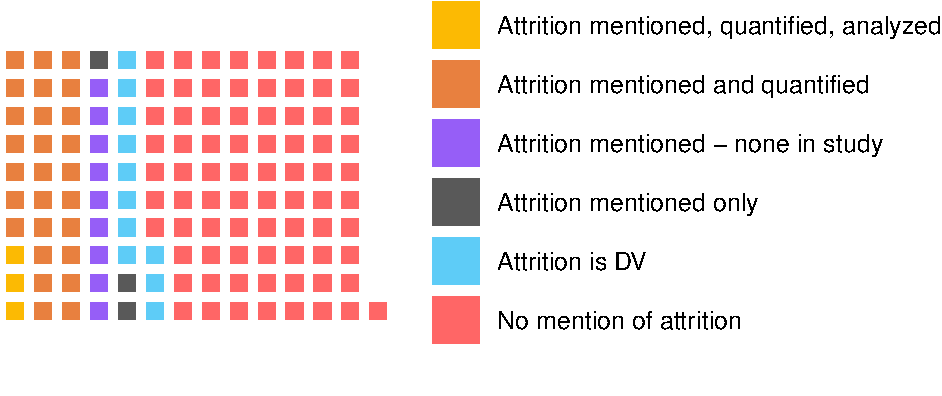
\includegraphics{paper_replication_files/figure-latex/waffle-1.pdf}

\hypertarget{figure-3-attrition-timeline-visualization}{%
\section{Figure 3: Attrition timeline
visualization}\label{figure-3-attrition-timeline-visualization}}

\begin{Shaded}
\begin{Highlighting}[]
\CommentTok{\#plot\_attrition() function. }
\NormalTok{plot\_attrition }\OtherTok{\textless{}{-}} \ControlFlowTok{function}\NormalTok{(data}
\NormalTok{                           ,}\AttributeTok{treatment\_a =} \ConstantTok{NULL}
\NormalTok{                           ,}\AttributeTok{treatment\_q =} \ConstantTok{NULL}
\NormalTok{                           ,}\AttributeTok{outcome\_q =} \ConstantTok{NULL}
\NormalTok{                           ,}\AttributeTok{mycolors=} \ConstantTok{NULL}
\NormalTok{                           ,}\AttributeTok{title =} \ConstantTok{NULL}\NormalTok{)}
\NormalTok{  \{ }
  \CommentTok{\#required packages}
  \FunctionTok{require}\NormalTok{(ggplot2)}
  \FunctionTok{require}\NormalTok{(viridis)}
  \FunctionTok{require}\NormalTok{(Hmisc)}
  \FunctionTok{require}\NormalTok{(dplyr)}
  \FunctionTok{require}\NormalTok{(ggrepel)}
  \FunctionTok{require}\NormalTok{(data.table)}

\CommentTok{\# rename the condition variable}
\NormalTok{data\_original}\OtherTok{\textless{}{-}}\NormalTok{data }\CommentTok{\#save this original data for reference}
\NormalTok{data2 }\OtherTok{\textless{}{-}} \FunctionTok{rename}\NormalTok{(data, }\AttributeTok{cond\_new =}\NormalTok{ treatment\_a) }\CommentTok{\#create \textasciigrave{}cond\_new\textasciigrave{} var based on conditions}
\NormalTok{data}\SpecialCharTok{$}\NormalTok{cond\_new}\OtherTok{\textless{}{-}}\NormalTok{data2}\SpecialCharTok{$}\NormalTok{cond\_new}

\CommentTok{\#split the dataset into a list by conditions}
\NormalTok{data\_split}\OtherTok{\textless{}{-}}\FunctionTok{split}\NormalTok{(data, }\FunctionTok{with}\NormalTok{(data, cond\_new), }\AttributeTok{drop =} \ConstantTok{TRUE}\NormalTok{)}

\CommentTok{\#for loop to account for attrition by condition}
\NormalTok{listofdfs }\OtherTok{\textless{}{-}} \FunctionTok{list}\NormalTok{() }
\ControlFlowTok{for}\NormalTok{ (i }\ControlFlowTok{in} \DecValTok{1}\SpecialCharTok{:}\FunctionTok{length}\NormalTok{(data\_split)) \{}
  \CommentTok{\#first remove the \textasciigrave{}cond\_new\textasciigrave{} var we created before}
\NormalTok{    df}\OtherTok{\textless{}{-}}\FunctionTok{as.data.frame}\NormalTok{(data\_split[i])}
\NormalTok{    df[}\FunctionTok{ncol}\NormalTok{(df)]}\OtherTok{\textless{}{-}}\ConstantTok{NULL}
  \CommentTok{\#for each missing value assign value 1, for complete response assign 0.}
\NormalTok{    df}\OtherTok{\textless{}{-}} \FunctionTok{apply}\NormalTok{(df,}\DecValTok{2}\NormalTok{,}\ControlFlowTok{function}\NormalTok{(x) \{}\FunctionTok{ifelse}\NormalTok{(}\FunctionTok{is.na}\NormalTok{(x),}\DecValTok{1}\NormalTok{,}\DecValTok{0}\NormalTok{)\})}
  \CommentTok{\#apply "skip\_to\_attrite" to get rid of skippers}
\NormalTok{    df}\OtherTok{\textless{}{-}}\FunctionTok{t}\NormalTok{(}\FunctionTok{apply}\NormalTok{(df,}\DecValTok{1}\NormalTok{,skip\_to\_attrite))}
  \CommentTok{\#sum the number of missing (minus skippers) per q}
\NormalTok{    df1}\OtherTok{\textless{}{-}} \FunctionTok{data.frame}\NormalTok{(}\FunctionTok{colSums}\NormalTok{(df))}
  \CommentTok{\#rename this variable \textasciigrave{}missing\textasciigrave{}}
    \FunctionTok{colnames}\NormalTok{(df1)}\OtherTok{\textless{}{-}} \StringTok{"missing"}
  \CommentTok{\#create variable \textasciigrave{}attrited\textasciigrave{}, rather than missing minus skippers}
\NormalTok{    df1}\SpecialCharTok{$}\NormalTok{attrited}\OtherTok{\textless{}{-}}\FunctionTok{c}\NormalTok{(df1[}\DecValTok{1}\NormalTok{,], df1[}\SpecialCharTok{{-}}\DecValTok{1}\NormalTok{,] }\SpecialCharTok{{-}}\NormalTok{ df1[}\SpecialCharTok{{-}}\FunctionTok{nrow}\NormalTok{(df1),])}
  \CommentTok{\#\textasciigrave{}prop\_q\textasciigrave{} = attrited / n entering into the question}
\NormalTok{    df1}\SpecialCharTok{$}\NormalTok{n\_prev}\OtherTok{\textless{}{-}} \FunctionTok{Lag}\NormalTok{(}\FunctionTok{nrow}\NormalTok{(df) }\SpecialCharTok{{-}} \FunctionTok{as.numeric}\NormalTok{(df1}\SpecialCharTok{$}\NormalTok{missing), }\SpecialCharTok{+}\DecValTok{1}\NormalTok{)}
\NormalTok{    df1}\SpecialCharTok{$}\NormalTok{n\_prev[}\DecValTok{1}\NormalTok{] }\OtherTok{\textless{}{-}} \FunctionTok{nrow}\NormalTok{(df)}
\NormalTok{    df1}\SpecialCharTok{$}\NormalTok{prop\_q }\OtherTok{\textless{}{-}} \FunctionTok{round}\NormalTok{(df1}\SpecialCharTok{$}\NormalTok{attrited}\SpecialCharTok{/}\NormalTok{df1}\SpecialCharTok{$}\NormalTok{n\_prev,}\DecValTok{2}\NormalTok{)}
  \CommentTok{\#\textasciigrave{}proportion\textasciigrave{}= attrited / starting N}
\NormalTok{    df1}\SpecialCharTok{$}\NormalTok{proportion }\OtherTok{\textless{}{-}} \FunctionTok{round}\NormalTok{(df1}\SpecialCharTok{$}\NormalTok{attrited}\SpecialCharTok{/}\FunctionTok{nrow}\NormalTok{(df),}\DecValTok{2}\NormalTok{)}
  \CommentTok{\#add variable for question name}
\NormalTok{    df1}\SpecialCharTok{$}\NormalTok{questions}\OtherTok{\textless{}{-}}\FunctionTok{colnames}\NormalTok{(data\_original)}
  \CommentTok{\#based on rownames per dataset, create \textasciigrave{}treatment\textasciigrave{} var}
\NormalTok{    df1}\SpecialCharTok{$}\NormalTok{treatment}\OtherTok{\textless{}{-}}\FunctionTok{rownames}\NormalTok{(df1)}
\NormalTok{    df1}\SpecialCharTok{$}\NormalTok{treatment}\OtherTok{\textless{}{-}}\FunctionTok{gsub}\NormalTok{(}\StringTok{"}\SpecialCharTok{\textbackslash{}\textbackslash{}}\StringTok{..*"}\NormalTok{,}\StringTok{""}\NormalTok{,df1}\SpecialCharTok{$}\NormalTok{treatment)}
  \CommentTok{\#remove rownames}
    \FunctionTok{rownames}\NormalTok{(df1) }\OtherTok{\textless{}{-}} \FunctionTok{c}\NormalTok{()}
  \CommentTok{\#save as a list}
\NormalTok{    listofdfs[[i]] }\OtherTok{\textless{}{-}}\NormalTok{ df1}
\NormalTok{\}}

\CommentTok{\#merge all datasets in the list}
\NormalTok{data\_combined}\OtherTok{\textless{}{-}} \FunctionTok{rbindlist}\NormalTok{(listofdfs)}

\CommentTok{\#create a vector for the unique values of the question names}
\NormalTok{question\_names}\OtherTok{\textless{}{-}}\FunctionTok{unique}\NormalTok{(data\_combined}\SpecialCharTok{$}\NormalTok{questions)}
\CommentTok{\#change question var to factor and numeric for plotting}
\NormalTok{data\_combined}\SpecialCharTok{$}\NormalTok{questions }\OtherTok{\textless{}{-}} \FunctionTok{factor}\NormalTok{(data\_combined}\SpecialCharTok{$}\NormalTok{questions,}
                                  \AttributeTok{levels=}\NormalTok{question\_names)}
\NormalTok{data\_combined}\SpecialCharTok{$}\NormalTok{questions2}\OtherTok{\textless{}{-}}\FunctionTok{as.numeric}\NormalTok{(data\_combined}\SpecialCharTok{$}\NormalTok{questions)}


\CommentTok{\#create indicators for Vlines}
\CommentTok{\#treatment Vline}
\NormalTok{treatment\_vars}\OtherTok{\textless{}{-}}\FunctionTok{as.data.frame}\NormalTok{(}\FunctionTok{match}\NormalTok{(treatment\_q, question\_names))}
\FunctionTok{colnames}\NormalTok{(treatment\_vars) }\OtherTok{\textless{}{-}} \StringTok{"treatment\_q"}
\NormalTok{treatment\_vars}\SpecialCharTok{$}\NormalTok{label}\OtherTok{\textless{}{-}}\StringTok{"Treatment Given"} \CommentTok{\#labels}
\NormalTok{treatment\_vars}\SpecialCharTok{$}\NormalTok{color}\OtherTok{\textless{}{-}} \StringTok{"black"} \CommentTok{\#color of vline}
\NormalTok{treatment\_vars}\SpecialCharTok{$}\NormalTok{ynum}\OtherTok{\textless{}{-}} \FloatTok{0.5} \CommentTok{\#where the label appears on yaxis}
\NormalTok{treatment\_vars}\SpecialCharTok{$}\NormalTok{size}\OtherTok{\textless{}{-}}\DecValTok{1}

\CommentTok{\#outcome Vline}
\NormalTok{DV}\OtherTok{\textless{}{-}}\FunctionTok{as.data.frame}\NormalTok{(}\FunctionTok{match}\NormalTok{(outcome\_q, question\_names))}
\FunctionTok{colnames}\NormalTok{(DV) }\OtherTok{\textless{}{-}} \StringTok{"outcome\_q"}
\NormalTok{DV}\SpecialCharTok{$}\NormalTok{label}\OtherTok{\textless{}{-}}\StringTok{"Outcome Question"}
\NormalTok{DV}\SpecialCharTok{$}\NormalTok{color}\OtherTok{\textless{}{-}} \StringTok{"gray48"}
\NormalTok{DV}\SpecialCharTok{$}\NormalTok{ynum}\OtherTok{\textless{}{-}} \FloatTok{0.5}
\NormalTok{DV}\SpecialCharTok{$}\NormalTok{size}\OtherTok{\textless{}{-}}\DecValTok{1}

\NormalTok{p }\OtherTok{\textless{}{-}}\NormalTok{ data\_combined }\SpecialCharTok{\%\textgreater{}\%}
      
    \FunctionTok{ggplot}\NormalTok{(}\FunctionTok{aes}\NormalTok{(questions2,prop\_q, }\AttributeTok{group =}\NormalTok{ treatment)) }\SpecialCharTok{+}
  
        \CommentTok{\#scale x axis from 1:10}
       \FunctionTok{scale\_x\_continuous}\NormalTok{(}\AttributeTok{breaks=}\FunctionTok{unique}\NormalTok{(data\_combined}\SpecialCharTok{$}\NormalTok{questions2),}
       \AttributeTok{labels=}\NormalTok{question\_names) }\SpecialCharTok{+} \CommentTok{\#label questions with Q}
   
      \CommentTok{\#create geomlines for \textasciigrave{}treatment\textasciigrave{} and \textasciigrave{}control\textasciigrave{} }
      \FunctionTok{geom\_line}\NormalTok{(}\AttributeTok{data =}\NormalTok{ data\_combined, }\FunctionTok{aes}\NormalTok{(questions2, prop\_q, }
                             \AttributeTok{color =}\NormalTok{ treatment, }
                             \AttributeTok{linetype=}\NormalTok{treatment),}
                \AttributeTok{size =} \FloatTok{1.1}\NormalTok{,}
                             \AttributeTok{show.legend =} \ConstantTok{FALSE}\NormalTok{) }\SpecialCharTok{+}
      
      \CommentTok{\#label \textasciigrave{}treatment\textasciigrave{} and \textasciigrave{}control\textasciigrave{}}

      \FunctionTok{geom\_text\_repel}\NormalTok{(}\AttributeTok{data =}\NormalTok{ data\_combined }\SpecialCharTok{\%\textgreater{}\%} \FunctionTok{filter}\NormalTok{(questions2 }\SpecialCharTok{==} \FunctionTok{length}\NormalTok{(question\_names)),}
                \FunctionTok{aes}\NormalTok{(}\AttributeTok{label =}\NormalTok{ treatment, }
                    \AttributeTok{x =}\NormalTok{ questions2, }
                    \AttributeTok{y =}\NormalTok{ prop\_q, }
                    \AttributeTok{color =}\NormalTok{ treatment),}
                \AttributeTok{min.segment.length =} \DecValTok{0}\NormalTok{,}
                    \AttributeTok{show.legend =} \ConstantTok{FALSE}\NormalTok{)}\SpecialCharTok{+}

     \CommentTok{\#add a geom\_point}
     \FunctionTok{geom\_point}\NormalTok{(}\AttributeTok{size=}\DecValTok{2}\NormalTok{, }\FunctionTok{aes}\NormalTok{(}\AttributeTok{colour=}\FunctionTok{factor}\NormalTok{(treatment), }
                            \AttributeTok{fill =} \FunctionTok{factor}\NormalTok{(treatment)), }\AttributeTok{show.legend =} \ConstantTok{FALSE}\NormalTok{) }

    \ControlFlowTok{if}\NormalTok{(}\SpecialCharTok{!}\FunctionTok{is.null}\NormalTok{(mycolors)) \{p }\OtherTok{\textless{}{-}}\NormalTok{ p}\SpecialCharTok{+} \FunctionTok{scale\_colour\_manual}\NormalTok{(}\AttributeTok{values=}\NormalTok{mycolors)\}}
    
     \CommentTok{\#make treatment red and control blue}
     
    \CommentTok{\#remove gray background}
\NormalTok{   p }\OtherTok{\textless{}{-}}\NormalTok{ p }\SpecialCharTok{+} \FunctionTok{theme}\NormalTok{(}\AttributeTok{panel.grid.major =} \FunctionTok{element\_blank}\NormalTok{(), }\AttributeTok{panel.grid.minor =} 
          \FunctionTok{element\_blank}\NormalTok{(), }\AttributeTok{panel.background =} \FunctionTok{element\_blank}\NormalTok{(), }
           \AttributeTok{axis.line =} \FunctionTok{element\_line}\NormalTok{(}\AttributeTok{colour =} \StringTok{"black"}\NormalTok{)) }\SpecialCharTok{+}
  
    \FunctionTok{ylim}\NormalTok{ (}\DecValTok{0}\NormalTok{, }\DecValTok{1}\NormalTok{) }\SpecialCharTok{+}
    \CommentTok{\# add title and labels to axis  }
    \FunctionTok{labs}\NormalTok{(}\AttributeTok{x =} \StringTok{"Survey Questions"}\NormalTok{, }\AttributeTok{y =} \StringTok{"Proportion of attrited"}\NormalTok{) }\SpecialCharTok{+}
    \FunctionTok{ggtitle}\NormalTok{(title)}

\CommentTok{\#add the vertical lines}
\NormalTok{a}\OtherTok{\textless{}{-}}\NormalTok{p }\SpecialCharTok{+}  
    \CommentTok{\#DV vertical lines}
    \FunctionTok{annotate}\NormalTok{(}\AttributeTok{geom =} \StringTok{"vline"}\NormalTok{,}
             \AttributeTok{x =} \FunctionTok{c}\NormalTok{(DV}\SpecialCharTok{$}\NormalTok{outcome\_q),}
             \AttributeTok{xintercept =} \FunctionTok{c}\NormalTok{(DV}\SpecialCharTok{$}\NormalTok{outcome\_q),}
             \AttributeTok{color =} \FunctionTok{c}\NormalTok{(DV}\SpecialCharTok{$}\NormalTok{color),}
             \AttributeTok{size =} \FunctionTok{c}\NormalTok{(DV}\SpecialCharTok{$}\NormalTok{size)) }\SpecialCharTok{+}
  
    \FunctionTok{annotate}\NormalTok{(}\AttributeTok{geom =} \StringTok{"text"}\NormalTok{,}
             \AttributeTok{label =} \FunctionTok{c}\NormalTok{(DV}\SpecialCharTok{$}\NormalTok{label),}
             \AttributeTok{x =} \FunctionTok{c}\NormalTok{(DV}\SpecialCharTok{$}\NormalTok{outcome\_q),}
             \AttributeTok{y =} \FunctionTok{c}\NormalTok{(DV}\SpecialCharTok{$}\NormalTok{ynum),}
             \AttributeTok{color =} \FunctionTok{c}\NormalTok{(DV}\SpecialCharTok{$}\NormalTok{color),}
             \AttributeTok{angle =} \DecValTok{90}\NormalTok{, }
             \AttributeTok{vjust =} \FloatTok{1.5}\NormalTok{) }\SpecialCharTok{+} 
  
   \CommentTok{\#treatments vertical lines}
   \FunctionTok{annotate}\NormalTok{(}\AttributeTok{geom =} \StringTok{"vline"}\NormalTok{,}
             \AttributeTok{x =} \FunctionTok{c}\NormalTok{(treatment\_vars}\SpecialCharTok{$}\NormalTok{treatment\_q),}
             \AttributeTok{xintercept =} \FunctionTok{c}\NormalTok{(treatment\_vars}\SpecialCharTok{$}\NormalTok{treatment\_q),}
             \AttributeTok{color =} \FunctionTok{c}\NormalTok{(treatment\_vars}\SpecialCharTok{$}\NormalTok{color),}
             \AttributeTok{size =} \FunctionTok{c}\NormalTok{(treatment\_vars}\SpecialCharTok{$}\NormalTok{size)) }\SpecialCharTok{+}
  
    \FunctionTok{annotate}\NormalTok{(}\AttributeTok{geom =} \StringTok{"text"}\NormalTok{,}
             \AttributeTok{label =} \FunctionTok{c}\NormalTok{(treatment\_vars}\SpecialCharTok{$}\NormalTok{label),}
             \AttributeTok{x =} \FunctionTok{c}\NormalTok{(treatment\_vars}\SpecialCharTok{$}\NormalTok{treatment\_q),}
             \AttributeTok{y =} \FunctionTok{c}\NormalTok{(treatment\_vars}\SpecialCharTok{$}\NormalTok{ynum),}
             \AttributeTok{color =} \FunctionTok{c}\NormalTok{(treatment\_vars}\SpecialCharTok{$}\NormalTok{color),}
             \AttributeTok{angle =} \DecValTok{90}\NormalTok{, }
             \AttributeTok{vjust =} \FloatTok{1.5}\NormalTok{)}
\FunctionTok{print}\NormalTok{(a)}
\NormalTok{\}  }
  


\CommentTok{\#Make toy plots for paper}
\FunctionTok{require}\NormalTok{(ggpattern)}

\CommentTok{\#(a) Low Level Attrition}
\CommentTok{\#Attition post{-}treatment (throughout survey)}
\NormalTok{n }\OtherTok{\textless{}{-}} \DecValTok{1000}
\NormalTok{df }\OtherTok{\textless{}{-}} \FunctionTok{data.frame}\NormalTok{(}
\AttributeTok{Q1 =} \FunctionTok{sample}\NormalTok{(}\FunctionTok{c}\NormalTok{(}\StringTok{"Treatment"}\NormalTok{, }\StringTok{"Control"}\NormalTok{), n, }\AttributeTok{rep =} \ConstantTok{TRUE}\NormalTok{), }\CommentTok{\#we will assume conditions are assigned when entering survey}
\AttributeTok{Q2 =} \FunctionTok{sample}\NormalTok{(}\FunctionTok{c}\NormalTok{(}\DecValTok{18}\SpecialCharTok{:}\DecValTok{90}\NormalTok{), n, }\AttributeTok{rep =} \ConstantTok{TRUE}\NormalTok{), }\CommentTok{\#age}
\AttributeTok{Q3 =} \FunctionTok{sample}\NormalTok{(}\FunctionTok{c}\NormalTok{(}\StringTok{"m"}\NormalTok{, }\StringTok{"f"}\NormalTok{), n, }\AttributeTok{rep =} \ConstantTok{TRUE}\NormalTok{, }\AttributeTok{prob =} \FunctionTok{c}\NormalTok{(}\FloatTok{0.55}\NormalTok{, }\FloatTok{0.45}\NormalTok{)), }\CommentTok{\#sex}
\AttributeTok{Q4 =} \FunctionTok{sample}\NormalTok{(}\FunctionTok{c}\NormalTok{(}\DecValTok{0}\NormalTok{,}\DecValTok{1}\NormalTok{), n, }\AttributeTok{rep =} \ConstantTok{TRUE}\NormalTok{))}\CommentTok{\#other general pre{-}treatment questions}
\NormalTok{df}\SpecialCharTok{$}\NormalTok{Q5 }\OtherTok{=}\NormalTok{ df}\SpecialCharTok{$}\NormalTok{Q1 }\CommentTok{\#at Q5 respondents are presented with treatment (say, vignette)}
\NormalTok{df}\SpecialCharTok{$}\NormalTok{Q6 }\OtherTok{=} \FunctionTok{sample}\NormalTok{(}\FunctionTok{c}\NormalTok{(}\DecValTok{0}\NormalTok{,}\DecValTok{1}\NormalTok{), n, }\AttributeTok{rep =} \ConstantTok{TRUE}\NormalTok{) }\CommentTok{\#post treatment questions}
\NormalTok{df}\SpecialCharTok{$}\NormalTok{Q7 }\OtherTok{=} \FunctionTok{sample}\NormalTok{(}\FunctionTok{c}\NormalTok{(}\DecValTok{0}\NormalTok{,}\DecValTok{1}\NormalTok{), n, }\AttributeTok{rep =} \ConstantTok{TRUE}\NormalTok{)}
\NormalTok{df}\SpecialCharTok{$}\NormalTok{Q8 }\OtherTok{=} \FunctionTok{sample}\NormalTok{(}\FunctionTok{c}\NormalTok{(}\DecValTok{0}\NormalTok{,}\DecValTok{1}\NormalTok{), n, }\AttributeTok{rep =} \ConstantTok{TRUE}\NormalTok{)}
\NormalTok{df}\SpecialCharTok{$}\NormalTok{Q9 }\OtherTok{=} \FunctionTok{sample}\NormalTok{(}\FunctionTok{c}\NormalTok{(}\DecValTok{0}\NormalTok{,}\DecValTok{1}\NormalTok{), n, }\AttributeTok{rep =} \ConstantTok{TRUE}\NormalTok{)}
\NormalTok{df}\SpecialCharTok{$}\NormalTok{Q10 }\OtherTok{=} \FunctionTok{sample}\NormalTok{(}\FunctionTok{c}\NormalTok{(}\DecValTok{0}\NormalTok{,}\DecValTok{1}\NormalTok{), n, }\AttributeTok{rep =} \ConstantTok{TRUE}\NormalTok{)}

\NormalTok{df\_a}\OtherTok{\textless{}{-}}\NormalTok{df}

\CommentTok{\#Generate attrition post}
\FunctionTok{invisible}\NormalTok{(}
\FunctionTok{sapply}\NormalTok{(}\FunctionTok{sample}\NormalTok{(}\DecValTok{1}\SpecialCharTok{:}\FunctionTok{nrow}\NormalTok{(df\_a), }\DecValTok{150}\NormalTok{),}\ControlFlowTok{function}\NormalTok{(x) \{}
\NormalTok{    a }\OtherTok{\textless{}{-}} \FunctionTok{sample}\NormalTok{(}\DecValTok{1}\SpecialCharTok{:}\DecValTok{10}\NormalTok{,}\DecValTok{1}\NormalTok{)}
\NormalTok{    df\_a[x,a}\SpecialCharTok{:}\FunctionTok{ncol}\NormalTok{(df\_a)] }\OtherTok{\textless{}\textless{}{-}} \ConstantTok{NA}
\NormalTok{\}}
\NormalTok{))}



\CommentTok{\#generate plot (a)}
\NormalTok{a}\OtherTok{\textless{}{-}}\FunctionTok{plot\_attrition}\NormalTok{(}\AttributeTok{data=}\NormalTok{df\_a,}
              \AttributeTok{treatment\_a =} \StringTok{"Q1"}\NormalTok{,}
              \AttributeTok{treatment\_q =} \StringTok{"Q5"}\NormalTok{,}
              \AttributeTok{outcome\_q =}  \FunctionTok{c}\NormalTok{(}\StringTok{"Q6"}\NormalTok{, }\StringTok{"Q7"}\NormalTok{),}
              \AttributeTok{title =} \StringTok{"(a) Low Level Attrition"}\NormalTok{,}
              \AttributeTok{mycolors =} \FunctionTok{c}\NormalTok{(}\StringTok{"\#000066"}\NormalTok{,}\StringTok{"\#CC0033"}\NormalTok{))}
\end{Highlighting}
\end{Shaded}

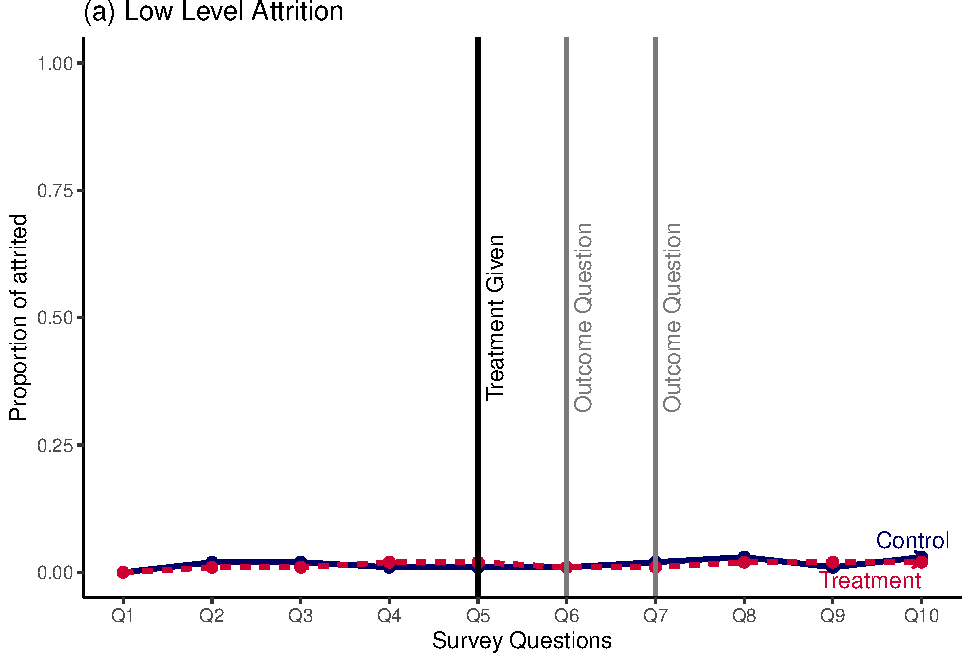
\includegraphics{paper_replication_files/figure-latex/timeline-1.pdf}

\begin{Shaded}
\begin{Highlighting}[]
\CommentTok{\#(b) Pre{-}treatment Attrition}
\NormalTok{df\_b}\OtherTok{\textless{}{-}}\NormalTok{df}
\CommentTok{\#Generate attrition pre{-}treatment}
\FunctionTok{invisible}\NormalTok{(}
\FunctionTok{sapply}\NormalTok{(}\FunctionTok{sample}\NormalTok{(}\DecValTok{1}\SpecialCharTok{:}\FunctionTok{nrow}\NormalTok{(df\_b), }\DecValTok{700}\NormalTok{),}\ControlFlowTok{function}\NormalTok{(x) \{}
\NormalTok{    a }\OtherTok{\textless{}{-}} \FunctionTok{sample}\NormalTok{(}\DecValTok{1}\SpecialCharTok{:}\DecValTok{4}\NormalTok{,}\DecValTok{1}\NormalTok{)}
\NormalTok{    df\_b[x,a}\SpecialCharTok{:}\FunctionTok{ncol}\NormalTok{(df\_b)] }\OtherTok{\textless{}\textless{}{-}} \ConstantTok{NA}
\NormalTok{\}}
\NormalTok{))}


\CommentTok{\#generate plot (b)}
\NormalTok{b}\OtherTok{\textless{}{-}}\FunctionTok{plot\_attrition}\NormalTok{(}\AttributeTok{data=}\NormalTok{df\_b,}
              \AttributeTok{treatment\_a =} \StringTok{"Q1"}\NormalTok{,}
              \AttributeTok{treatment\_q =} \StringTok{"Q5"}\NormalTok{,}
              \AttributeTok{outcome\_q =}  \FunctionTok{c}\NormalTok{(}\StringTok{"Q6"}\NormalTok{, }\StringTok{"Q7"}\NormalTok{),}
              \AttributeTok{title =} \StringTok{"(b) Pre{-}treatment Attrition"}\NormalTok{,}
              \AttributeTok{mycolors =} \FunctionTok{c}\NormalTok{(}\StringTok{"\#000066"}\NormalTok{,}\StringTok{"\#CC0033"}\NormalTok{))}
\end{Highlighting}
\end{Shaded}

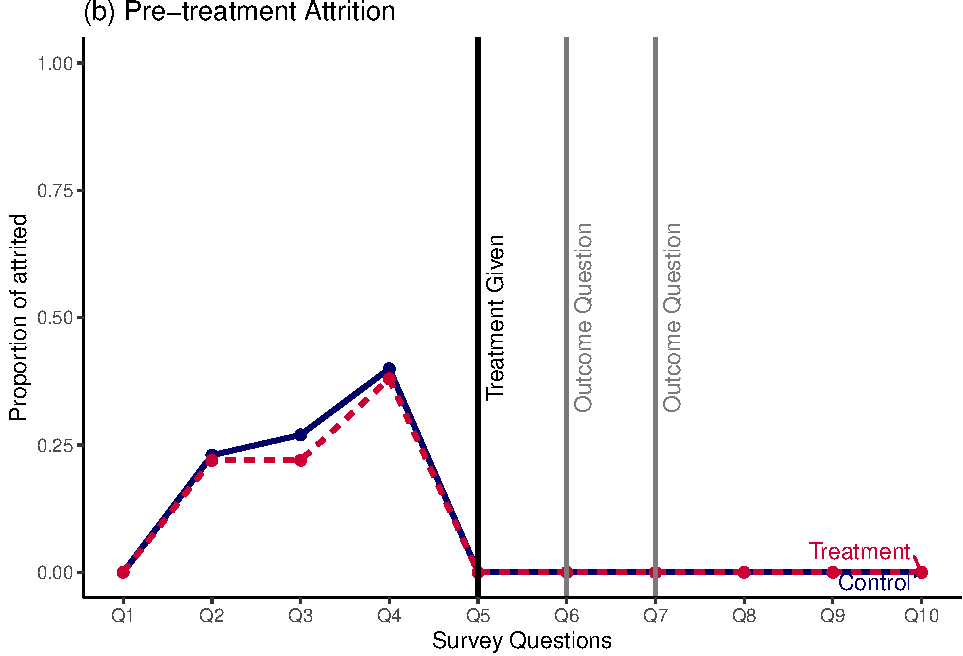
\includegraphics{paper_replication_files/figure-latex/timeline-2.pdf}

\begin{Shaded}
\begin{Highlighting}[]
\CommentTok{\#(c) Post{-}treatment Attrition (immediate)}
\NormalTok{df\_c}\OtherTok{\textless{}{-}}\NormalTok{df}

\CommentTok{\#First, we generate some general attrition at treatment}
\FunctionTok{invisible}\NormalTok{(}
\FunctionTok{sapply}\NormalTok{(}\FunctionTok{sample}\NormalTok{(}\DecValTok{1}\SpecialCharTok{:}\FunctionTok{nrow}\NormalTok{(df\_c), }\DecValTok{500}\NormalTok{, }\FloatTok{0.8}\SpecialCharTok{*}\FunctionTok{nrow}\NormalTok{(df\_c)),}\ControlFlowTok{function}\NormalTok{(x) \{}
\NormalTok{    a }\OtherTok{\textless{}{-}} \FunctionTok{sample}\NormalTok{(}\DecValTok{5}\SpecialCharTok{:}\DecValTok{6}\NormalTok{,}\DecValTok{1}\NormalTok{)}
\NormalTok{    df\_c[x,a}\SpecialCharTok{:}\FunctionTok{ncol}\NormalTok{(df\_c)] }\OtherTok{\textless{}\textless{}{-}} \ConstantTok{NA}
\NormalTok{\}}
\NormalTok{))}

\CommentTok{\#second, we add some attrition that\textquotesingle{}s correlated with the treatment}
\CommentTok{\#specifically, we want to demonstrate attrition that happens at a certain time }
\CommentTok{\#to do so, we add a running var that will demonstrate time}
\NormalTok{df\_c}\SpecialCharTok{$}\NormalTok{no}\OtherTok{\textless{}{-}}\FunctionTok{rownames}\NormalTok{(df\_c)}
\NormalTok{df\_c}\SpecialCharTok{$}\NormalTok{Q6}\OtherTok{\textless{}{-}}\FunctionTok{ifelse}\NormalTok{(df\_c}\SpecialCharTok{$}\NormalTok{Q5}\SpecialCharTok{==}\StringTok{"Treatment"}\SpecialCharTok{\&}\NormalTok{(df\_c}\SpecialCharTok{$}\NormalTok{no}\SpecialCharTok{\textgreater{}}\DecValTok{100}\SpecialCharTok{\&}\NormalTok{df\_c}\SpecialCharTok{$}\NormalTok{no}\SpecialCharTok{\textless{}}\DecValTok{300}\NormalTok{), }\ConstantTok{NA}\NormalTok{,df\_c}\SpecialCharTok{$}\NormalTok{Q6)}
\NormalTok{df\_c}\SpecialCharTok{$}\NormalTok{Q7}\OtherTok{\textless{}{-}}\FunctionTok{ifelse}\NormalTok{(}\FunctionTok{is.na}\NormalTok{(df\_c}\SpecialCharTok{$}\NormalTok{Q6),}\ConstantTok{NA}\NormalTok{,df\_c}\SpecialCharTok{$}\NormalTok{Q7)}
\NormalTok{df\_c}\SpecialCharTok{$}\NormalTok{Q8}\OtherTok{\textless{}{-}}\FunctionTok{ifelse}\NormalTok{(}\FunctionTok{is.na}\NormalTok{(df\_c}\SpecialCharTok{$}\NormalTok{Q6),}\ConstantTok{NA}\NormalTok{,df\_c}\SpecialCharTok{$}\NormalTok{Q8)}
\NormalTok{df\_c}\SpecialCharTok{$}\NormalTok{Q9}\OtherTok{\textless{}{-}}\FunctionTok{ifelse}\NormalTok{(}\FunctionTok{is.na}\NormalTok{(df\_c}\SpecialCharTok{$}\NormalTok{Q6),}\ConstantTok{NA}\NormalTok{,df\_c}\SpecialCharTok{$}\NormalTok{Q9)}
\NormalTok{df\_c}\SpecialCharTok{$}\NormalTok{Q10}\OtherTok{\textless{}{-}}\FunctionTok{ifelse}\NormalTok{(}\FunctionTok{is.na}\NormalTok{(df\_c}\SpecialCharTok{$}\NormalTok{Q6),}\ConstantTok{NA}\NormalTok{,df\_c}\SpecialCharTok{$}\NormalTok{Q10)}

\NormalTok{df\_c}\SpecialCharTok{$}\NormalTok{no}\OtherTok{\textless{}{-}}\ConstantTok{NULL}

\CommentTok{\#generate plot (c)}
\NormalTok{c}\OtherTok{\textless{}{-}}\FunctionTok{plot\_attrition}\NormalTok{(}\AttributeTok{data=}\NormalTok{df\_c,}
              \AttributeTok{treatment\_a =} \StringTok{"Q1"}\NormalTok{,}
              \AttributeTok{treatment\_q =} \StringTok{"Q5"}\NormalTok{,}
              \AttributeTok{outcome\_q =}  \FunctionTok{c}\NormalTok{(}\StringTok{"Q6"}\NormalTok{, }\StringTok{"Q7"}\NormalTok{),}
              \AttributeTok{title =} \StringTok{"(c) Post{-}treatment Attrition (immediate)"}\NormalTok{,}
              \AttributeTok{mycolors =} \FunctionTok{c}\NormalTok{(}\StringTok{"\#000066"}\NormalTok{,}\StringTok{"\#CC0033"}\NormalTok{))}
\end{Highlighting}
\end{Shaded}

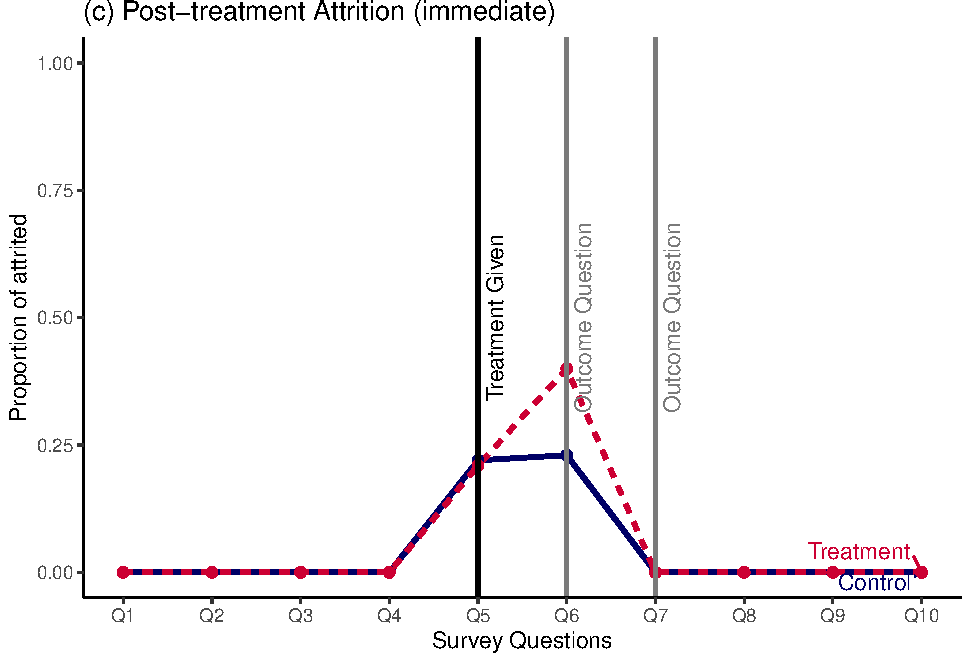
\includegraphics{paper_replication_files/figure-latex/timeline-3.pdf}

\begin{Shaded}
\begin{Highlighting}[]
\CommentTok{\#(d) Post{-}treatment Attrition (prolonged)}
\NormalTok{df\_d}\OtherTok{\textless{}{-}}\NormalTok{df}
\CommentTok{\#Generate attrition at DV + after}
\FunctionTok{invisible}\NormalTok{(}
\FunctionTok{sapply}\NormalTok{(}\FunctionTok{sample}\NormalTok{(}\DecValTok{1}\SpecialCharTok{:}\FunctionTok{nrow}\NormalTok{(df\_d), }\DecValTok{700}\NormalTok{),}\ControlFlowTok{function}\NormalTok{(x) \{}
\NormalTok{    a }\OtherTok{\textless{}{-}} \FunctionTok{sample}\NormalTok{(}\DecValTok{6}\SpecialCharTok{:}\DecValTok{10}\NormalTok{,}\DecValTok{1}\NormalTok{)}
\NormalTok{    df\_d[x,a}\SpecialCharTok{:}\FunctionTok{ncol}\NormalTok{(df\_d)] }\OtherTok{\textless{}\textless{}{-}} \ConstantTok{NA}
\NormalTok{\}}
\NormalTok{))}

\CommentTok{\#generate plot (d)}
\NormalTok{d}\OtherTok{\textless{}{-}}\FunctionTok{plot\_attrition}\NormalTok{(}\AttributeTok{data=}\NormalTok{df\_d,}
              \AttributeTok{treatment\_a =} \StringTok{"Q1"}\NormalTok{,}
              \AttributeTok{treatment\_q =} \StringTok{"Q5"}\NormalTok{,}
              \AttributeTok{outcome\_q =}  \FunctionTok{c}\NormalTok{(}\StringTok{"Q6"}\NormalTok{, }\StringTok{"Q7"}\NormalTok{),}
              \AttributeTok{title =} \StringTok{"(d) Post{-}treatment Attrition (prolonged)"}\NormalTok{,}
              \AttributeTok{mycolors =} \FunctionTok{c}\NormalTok{(}\StringTok{"\#000066"}\NormalTok{,}\StringTok{"\#CC0033"}\NormalTok{))}
\end{Highlighting}
\end{Shaded}

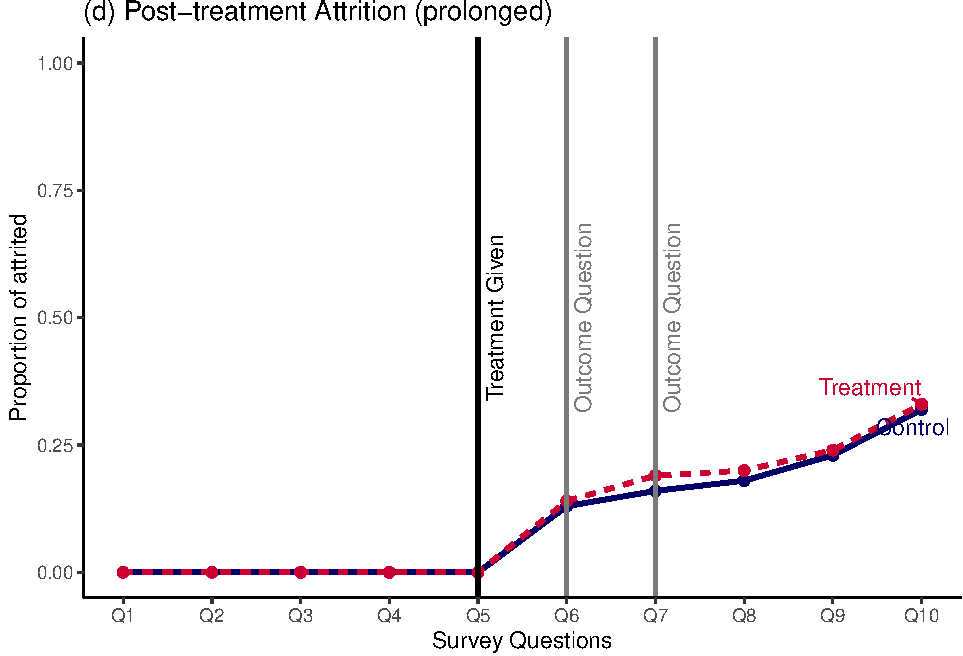
\includegraphics{paper_replication_files/figure-latex/timeline-4.pdf}

\begin{Shaded}
\begin{Highlighting}[]
\FunctionTok{require}\NormalTok{(grid)}

\NormalTok{figure }\OtherTok{\textless{}{-}} \FunctionTok{ggarrange}\NormalTok{(a }\SpecialCharTok{+} \FunctionTok{rremove}\NormalTok{(}\StringTok{"ylab"}\NormalTok{) }\SpecialCharTok{+} \FunctionTok{rremove}\NormalTok{(}\StringTok{"xlab"}\NormalTok{), b }\SpecialCharTok{+} \FunctionTok{rremove}\NormalTok{(}\StringTok{"ylab"}\NormalTok{) }
                    \SpecialCharTok{+} \FunctionTok{rremove}\NormalTok{(}\StringTok{"xlab"}\NormalTok{), c }\SpecialCharTok{+} \FunctionTok{rremove}\NormalTok{(}\StringTok{"ylab"}\NormalTok{) }\SpecialCharTok{+} \FunctionTok{rremove}\NormalTok{(}\StringTok{"xlab"}\NormalTok{), }
\NormalTok{                    d }\SpecialCharTok{+} \FunctionTok{rremove}\NormalTok{(}\StringTok{"ylab"}\NormalTok{) }\SpecialCharTok{+} \FunctionTok{rremove}\NormalTok{(}\StringTok{"xlab"}\NormalTok{), }\CommentTok{\# remove axis labels from plots}
                    \AttributeTok{labels =} \ConstantTok{NULL}\NormalTok{,}
                    \AttributeTok{ncol =} \DecValTok{2}\NormalTok{, }\AttributeTok{nrow =} \DecValTok{2}\NormalTok{,}
                    \AttributeTok{common.legend =} \ConstantTok{TRUE}\NormalTok{, }\AttributeTok{legend =} \StringTok{"top"}\NormalTok{,}
                    \AttributeTok{align =} \StringTok{"hv"}\NormalTok{, }
                    \AttributeTok{font.label =} \FunctionTok{list}\NormalTok{(}\AttributeTok{size =} \DecValTok{10}\NormalTok{, }\AttributeTok{color =} \StringTok{"black"}\NormalTok{, }\AttributeTok{face =} \StringTok{"bold"}\NormalTok{, }
                                      \AttributeTok{family =} \ConstantTok{NULL}\NormalTok{, }\AttributeTok{position =} \StringTok{"top"}\NormalTok{))}

\FunctionTok{annotate\_figure}\NormalTok{(figure, }\AttributeTok{left =} \FunctionTok{textGrob}\NormalTok{(}\StringTok{"Proportion of attrited"}\NormalTok{, }\AttributeTok{rot =} \DecValTok{90}\NormalTok{, }\AttributeTok{vjust =} \DecValTok{1}\NormalTok{, }\AttributeTok{gp =} \FunctionTok{gpar}\NormalTok{(}\AttributeTok{cex =} \FloatTok{1.5}\NormalTok{)),}
                    \AttributeTok{bottom =} \FunctionTok{textGrob}\NormalTok{(}\StringTok{"Experiment Questions"}\NormalTok{, }\AttributeTok{gp =} \FunctionTok{gpar}\NormalTok{(}\AttributeTok{cex =} \FloatTok{1.5}\NormalTok{)))}
\end{Highlighting}
\end{Shaded}

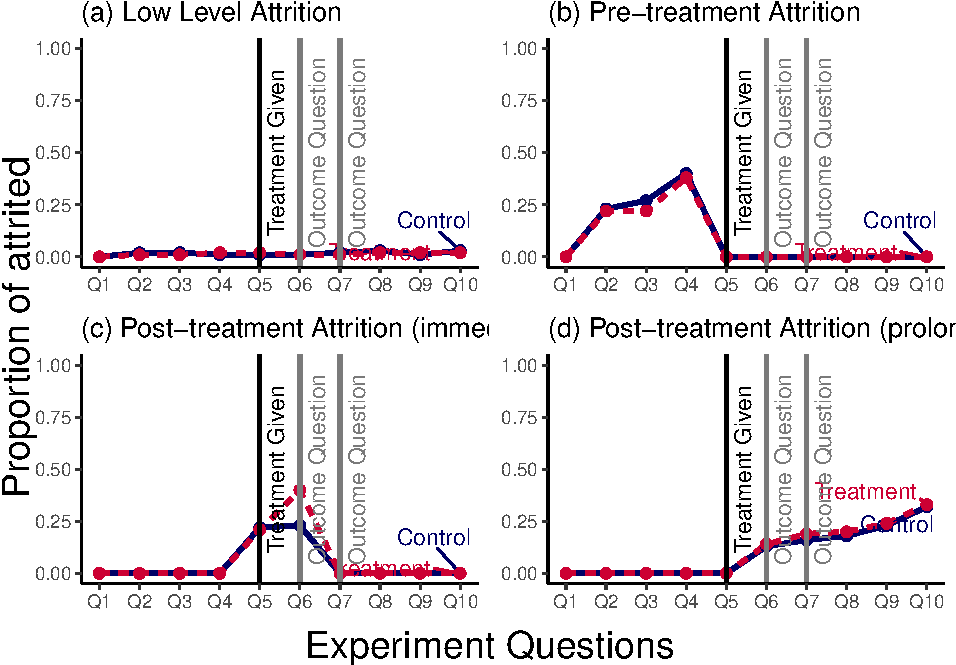
\includegraphics{paper_replication_files/figure-latex/timeline-5.pdf}

\begin{Shaded}
\begin{Highlighting}[]
\FunctionTok{vis\_miss\_treat}\NormalTok{(}\AttributeTok{data=}\NormalTok{df\_c,}
               \AttributeTok{treatment =} \StringTok{"Q5"}\NormalTok{)}
\end{Highlighting}
\end{Shaded}

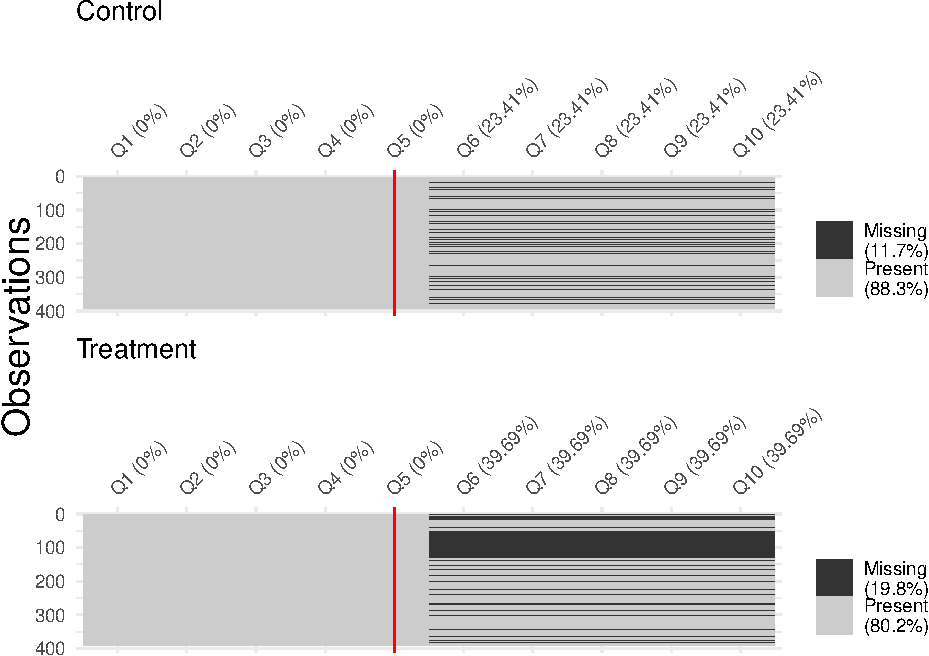
\includegraphics{paper_replication_files/figure-latex/timeline-6.pdf}

\end{document}
